\documentclass{standalone}
\usepackage[T1]{fontenc}
\usepackage{amsmath}
\usepackage{tikz}
\usetikzlibrary{arrows.meta}

\begin{document}
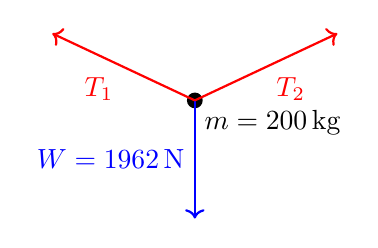
\begin{tikzpicture}
  % Coordinate system
% \draw[->, thick] (0,0) -- (1,0) node[right] {$x$};
% \draw[->, thick] (0,0) -- (0,1) node[above] {$y$};

  % Mass (represented as a point mass)
  \fill (0,0) circle (0.1) node[below right] {$m = 200\,\text{kg}$};

  % Forces
  \draw[->, thick, blue] (0,0) -- (0,-1.5) node[midway, left] {$W = 1962\,\text{N}$};
  \draw[->, thick, red] (0,0) -- (-1.81,0.85) node[midway, below left] {$T_1$};
  \draw[->, thick, red] (0,0) -- (1.81,0.85) node[midway, below right] {$T_2$};
 % \draw[->, thick, red] (0,0) -- (0,2) node[midway, right] {$T_3$};
\end{tikzpicture}
\end{document}
